\documentclass[11pt,a4paper]{article}

\usepackage[utf8]{inputenc}
\usepackage[T1]{fontenc}
\usepackage{lmodern}
\usepackage[margin=2.5cm]{geometry}
\usepackage{graphicx}
\usepackage{booktabs}
\usepackage{tabularx}
\usepackage{xcolor}
\usepackage{listings}
\usepackage{enumitem}
\usepackage{pdflscape}
\usepackage{array}
\usepackage{tikz}
\usetikzlibrary{positioning,arrows.meta,fit,backgrounds}
\usepackage[hidelinks]{hyperref}

% ------------------------------------------------------------------
% Helpers
% ------------------------------------------------------------------
% Marks information that still has to be confirmed before release.
\newcommand{\tbd}[1]{\textcolor{red}{[TBD: #1]}}

% Includes an image when the file exists, otherwise draws a placeholder box.
\newcommand{\optionalimage}[3]{%
  \IfFileExists{#2}{\includegraphics[#1]{#2}}{%
    \fbox{\parbox[c][3cm][c]{0.6\linewidth}{\centering\small Placeholder: #3\\\texttt{\detokenize{#2}}}}}}

\lstdefinelanguage{json}{
  basicstyle=\ttfamily\footnotesize,
  showstringspaces=false,
  breaklines=true,
  string=[s]{"}{"},
  stringstyle=\color{blue!60!black},
  morecomment=[l]{//},
  commentstyle=\color{gray}
}
\lstset{frame=single,framerule=0.4pt,rulecolor=\color{gray!60},
        xleftmargin=2pt,xrightmargin=2pt}

\setlist{itemsep=2pt,topsep=4pt}

\title{\textbf{ESE Health Programming Challenge 2026-2027}}
\author{}
\date{}

\begin{document}

\maketitle
\vspace{-2.5em}
\noindent\textit{v1.0 Nov 5, 2026}\\
\textbf{Case:} Scenario-Driven Patient Simulation for Advanced Life Support training,
together with UMC Utrecht Wilhelmina Children's Hospital

\begin{itemize}
  \item \textbf{\href{https://forms.cloud.microsoft/e/8ff4475CMc}{Click here to enroll your group}} (Groups for Prog 6)
\end{itemize}

% ==================================================================
\section{Partners}
% ==================================================================
The partners in this challenge are:

\begin{center}
  \raisebox{-0.5\height}{
\includegraphics[height=1.7cm]{logos/umcu_wkz.png}}%
  \hspace{1.5cm}%
  \raisebox{-0.5\height}{\begin{tabular}{@{}l@{}}
    
\includegraphics[height=2.6cm]{logos/han.png}\\[1pt]
    \resizebox{3.93cm}{!}{\sffamily\bfseries HEALTH CONCEPT LAB}
  \end{tabular}}
\end{center}

\subsection*{Introduction}
Wilhelmina Children's Hospital (WKZ) in Utrecht, part of UMC Utrecht, is always
looking for new ways to improve the skills of its nurses and physicians.
Together with the HAN Health Concept Lab it develops tools for life support
training, including a manikin to practice high quality CardioPulmonary
Resuscitation (CPR).

In earlier years, teams built a simulated patient monitor on dedicated
simulation hardware. That monitor showed a patient frozen in one state, and the
hardware needed too much maintenance. This year the case stays close to WKZ,
but the hardware is small, cheap and replaceable, so your results remain usable
after the course. A real patient changes: without treatment a child
deteriorates, with the right treatment at the right time the child recovers.
This year you make the simulated patient come alive, with a scenario editor, a
scenario engine and a hacked thermometer.

% ==================================================================
\section{Case}
% ==================================================================
WKZ wants trainers to run complete clinical scenarios on the manikin,
without a technician behind a laptop changing numbers by hand. A scenario
describes how a pediatric patient develops: an onset, a path to recovery when
the team acts correctly, and a path to deterioration when it does not.

Three parties meet in such a training:
\begin{itemize}
  \item \textbf{The nursing instructor} designs the scenario: the patient
        states, the vital signs per state and which interventions move the
        patient from one state to another. The instructor is not a programmer.
  \item \textbf{The nurse in training} measures the vital signs with
        simulated devices and performs interventions, such as giving a
        medication or oxygen.
  \item \textbf{The instructor view} shows the instructor what is going on:
        the current state, the vital signs, the measurements and the
        interventions that were performed. There is no patient monitor this
        year.
\end{itemize}

Interventions can be \textbf{detected} and \textbf{simulated}. Detected means
that the system recognizes what the nurse does without anybody typing it in:
actions are detected by SimDevices or NFC-tagged cards. Simulated means that an intervention is entered by hand,
for example by the instructor when the nurse says ``I give oxygen'' and there is
no device for it, or by a virtual SimDevice. Both kinds move the scenario in
the same way. Detected interventions are also input for the instructor: what
the nurse actually did, and when, is shown live and in the debrief.

Resuscitation is more than compressions and ventilations. Around the patient,
nurses use
everyday devices: a thermometer, an AED, medication, a stethoscope. WKZ and the
HAN Health Concept Lab call these \textbf{SimDevices}. To the nurse a SimDevice
looks and works like the real thing, but it shows the values and behavior that
the scenario dictates, and it reports everything the nurse does with it.
Diagnosis and treatment then become part of the scenario, instead of the
trainer saying ``the temperature is now 39.5 degrees''. Every action,
measurement and medication ends up with a timestamp in one timeline for the
debrief.

A SimDevice is an \textbf{abstraction}: something that accepts commands from
the scenario and reports events. How it is realized does not matter to the
scenario engine. It can be a physical device with a small microcontroller
inside (BLE or Wi-Fi) or a virtual device on a screen. What the nurse does is detected with buttons,
sensors or NFC, for example a tagged syringe, AED pads or a stethoscope that
detect where they are placed. This year
three SimDevices take part, keep all three simple:
\begin{itemize}
  \item \textbf{Thermometer}: a donor infrared thermometer with a new
        microcontroller inside. It shows the body temperature from the
        scenario at the moment the trigger is pulled.
  \item \textbf{AED}: analyzes the rhythm of the current state and gives a
        shock. It is not yet certain that a physical AED will be available, so
        each group can also use a virtual one.
  \item \textbf{Medication}: for example NFC-tagged syringes. Scanning a
        syringe at the manikin tells the scenario which drug and which dose was
        given.
\end{itemize}

\paragraph{What you build.} Each team works on two sides of the system:
\begin{itemize}
  \item \textbf{Pi side}: a scenario editor for the instructor, the scenario
        engine and the instructor view.
  \item \textbf{Device side}: hack a donor thermometer into a SimDevice, with
        firmware written as a clean object oriented library that the next
        SimDevice can reuse.
\end{itemize}
Both sides meet via MQTT on the Pi.

Time is compressed: in a hospital a child may deteriorate over hours, in
training this happens within minutes. The compression ratio is part of the
scenario, so the instructor chooses it.

Remember what you are building. The analog world is non-deterministic and has
infinitely many states: a real patient is never in exactly the same state twice.
Real problems like this one cannot be exhaustively proven. A computer works
discretely, by assuming a perfectly discrete world. Your scenario engine is
therefore a deliberate, finite approximation of a patient. Good engineering
makes that approximation convincing for the nurse and transparent for the
instructor.

% ==================================================================
\section{Requirements}
% ==================================================================
WKZ wants to:
\begin{itemize}
  \item Run a scenario that changes the vital signs over time and in reaction
        to interventions.
  \item Detect interventions where possible, and simulate them where no
        detection exists, so the instructor always sees what was done.
  \item Let nursing instructors create and change scenarios without writing code.
  \item Run everything on a Raspberry Pi, also when no external network
        connection is available (hotspot mode).
\end{itemize}

Table~\ref{tab:moscow} lists the features with their MoSCoW priority.
Code quality and the number of features all add up to the final result.

\begin{table}[h]
\centering
\small
\begin{tabularx}{\linewidth}{@{}l X l@{}}
\toprule
\textbf{Priority} & \textbf{Feature} & \textbf{Difficulty} \\
\midrule
Must   & Scenario engine: loads a scenario from JSON and runs it as a state machine with time-based transitions & moderate \\
Must   & Scenario editor: an instructor creates and changes a scenario without editing JSON & moderate \\
Must   & The engine publishes the state and vital signs via MQTT & easy \\
Must   & Thermometer SimDevice: shows the scenario temperature when the trigger is pulled and reports the measurement via MQTT & difficult \\
Must   & Firmware as an OO library: display, buzzer, trigger and connection as classes behind interfaces & moderate \\
Should & Intervention-triggered transitions, detected via SimDevices or NFC cards (e.g.\ epinephrine card) & moderate \\
Should & Simulated interventions: the instructor enters an intervention on the instructor view when no detection exists & easy \\
Should & Smooth transitions between states (interpolation instead of jumps) & moderate \\
Should & Instructor view on the Pi screen: current state, vital signs, measurements and interventions & moderate \\
Should & Dutch PEWS score with color coding and risk group on the instructor view & moderate \\
Should & Debrief: timeline of states, interventions (marked detected or simulated) and SimDevice events with timing feedback & easy \\
Should & SimDevice abstraction: the engine works with every SimDevice through one interface, physical or virtual & moderate \\
Should & Thermometer mimics the original: start-up screen, measuring time, beeps, fever indication, buttons & moderate \\
Should & Virtual AED: analyzes the rhythm of the current state, advises a shock or not, and reports a delivered shock & moderate \\
Could  & Medication SimDevice, e.g.\ via NFC: tagged syringes identify drug and dose & moderate \\
Could  & Firmware on Zephyr RTOS & difficult \\
Could  & BLE connection via a gateway: gateway firmware plus gateway bridge on the Pi & difficult \\
Could  & Rhythm per state (e.g.\ sinus tachycardia, ventricular fibrillation) for the AED & easy \\
Could  & Design (on paper) how a physical AED would replace the virtual AED. Connecting it only if one is available & easy \\
Could  & Design a new SimDevice with the same library, e.g.\ a stethoscope with NFC auscultation points, a capnograph or a glucose meter & moderate \\
Won't  & Real patient data, certification as a medical device & \\
\bottomrule
\end{tabularx}
\caption{Feature priorities (MoSCoW).}
\label{tab:moscow}
\end{table}

% ==================================================================
\section{The Challenge}
% ==================================================================
\subsection{Architecture}
Your assignment is to program (parts) of this system. Figure~\ref{fig:arch}
shows the intended architecture. All components communicate via an MQTT broker
on the Raspberry Pi, so a team can replace one component without touching the
others.

\begin{figure}[h]
\centering
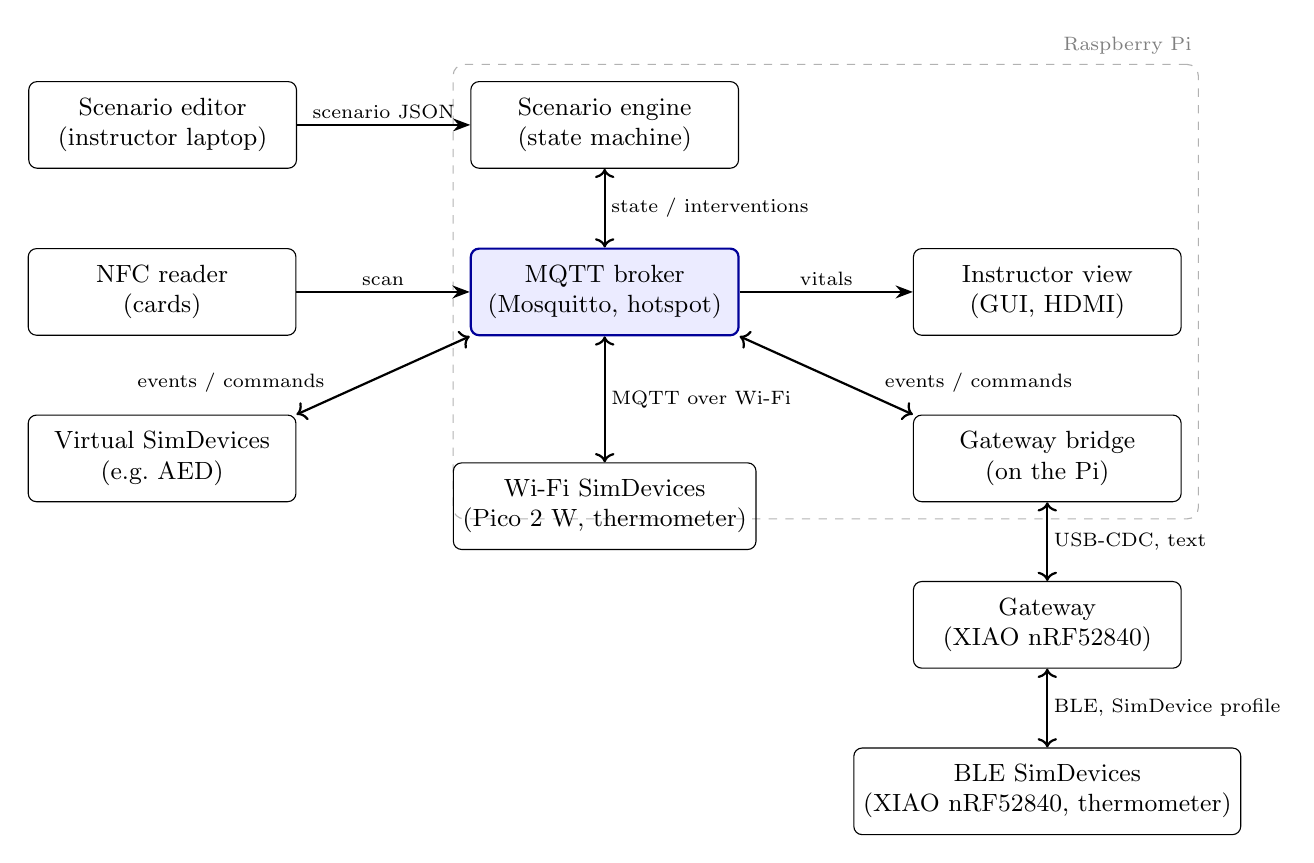
\begin{tikzpicture}[
  node distance=10mm and 22mm,
  box/.style={draw,rounded corners=3pt,align=center,minimum width=3.4cm,minimum height=1.1cm,font=\small},
  core/.style={box,fill=blue!8,draw=blue!60!black,thick},
  arr/.style={-{Stealth[length=2.2mm]},thick},
  lbl/.style={font=\scriptsize,midway,inner sep=2pt}
]
  \node[core] (broker) {MQTT broker\\(Mosquitto, hotspot)};
  \node[box, above=of broker] (engine) {Scenario engine\\(state machine)};
  \node[box, left=22mm of engine] (author) {Scenario editor\\(instructor laptop)};
  \node[box, right=of broker] (monitor) {Instructor view\\(GUI, HDMI)};
  \node[box, below=16mm of broker] (wifi) {Wi-Fi SimDevices\\(Pico 2 W, thermometer)};
  \node[box, left=22mm of broker] (nfc) {NFC reader\\(cards)};
  \node[box, below=of nfc] (virt) {Virtual SimDevices\\(e.g.\ AED)};
  \draw[arr,<->] (virt.north east) -- node[lbl,pos=0.2,above left]{events / commands} (broker.south west);
  \node[box, below=of monitor] (gwbridge) {Gateway bridge\\(on the Pi)};
  \node[box, below=of gwbridge] (gateway) {Gateway\\(XIAO nRF52840)};
  \node[box, below=of gateway] (simdev) {BLE SimDevices\\(XIAO nRF52840, thermometer)};

  \draw[arr,<->] (broker.south east) -- node[lbl,pos=0.8,above right]{events / commands} (gwbridge.north west);
  \draw[arr,<->] (gwbridge) -- node[lbl,right]{USB-CDC, text} (gateway);
  \draw[arr,<->] (gateway) -- node[lbl,right]{BLE, SimDevice profile} (simdev);

  \draw[arr] (author) -- node[lbl,above]{scenario JSON} (engine);
  \draw[arr,<->] (engine) -- node[lbl,right]{state / interventions} (broker);
  \draw[arr] (broker) -- node[lbl,above]{vitals} (monitor);
  \draw[arr] (nfc) -- node[lbl,above]{scan} (broker);
  \draw[arr,<->] (wifi) -- node[lbl,right]{MQTT over Wi-Fi} (broker);

  \begin{scope}[on background layer]
    \node[draw=gray!60,dashed,rounded corners=4pt,inner sep=6pt,
          fit=(engine)(broker)(monitor)(gwbridge),label={[font=\scriptsize,gray]above right:Raspberry Pi}] {};
  \end{scope}
\end{tikzpicture}
\caption{System architecture. Every component is a separate MQTT node. A physical SimDevice connects either directly over Wi-Fi or via a BLE gateway.}
\label{fig:arch}
\end{figure}

\subsection{High Level}
On the Raspberry Pi and for the user interfaces you may use any programming
language you like, as long as it runs on the Pi and talks MQTT. Because every
component is a separate MQTT node, components written in different languages
work together without problems. Whatever language you choose, use the Object
Oriented Paradigm, optimized for code quality. Please use the \textbf{Open-Closed principle}: adding
a new scenario, vital sign, intervention or scoring table must not require
changes to existing classes. Code is read more than ten times as often as it is
written, so naming, structure and comments count as much as features.

The instructor view is meant for the instructor, not for the nurse. It has to
be readable at a glance from a few meters away, during a busy scenario.

\subsection{Device Side: an OO Firmware Library}
The thermometer firmware is more than a one-off hack: write it as a reusable
object oriented library, so the next team can build a stethoscope or a glucose
meter on top of it. Model each part of the hardware as a class behind an
interface, for example a display, a buzzer, a backlight, a trigger or button,
and a connection to the Pi. A \texttt{Thermometer} class then only combines
these parts and implements the behavior of the device. Replacing the connection
(Wi-Fi or BLE) or the display driver must not change the \texttt{Thermometer}
class. Again: code is read more than ten times as often as it is written.

\paragraph{Microcontroller.} Two options fit this project:

\begin{table}[h]
\centering
\small
\begin{tabularx}{\linewidth}{@{}l >{\raggedright\arraybackslash}X >{\raggedright\arraybackslash}X@{}}
\toprule
 & \textbf{Seeed XIAO nRF52840 (Sense)} & \textbf{Raspberry Pi Pico 2 W} \\
\midrule
Size & 21 $\times$ 17.8~mm, fits in a thermometer & 51 $\times$ 21~mm, check the fit \\
Connection & BLE, via a gateway to the Pi & Wi-Fi, MQTT directly to the broker on the Pi \\
Power & very low, runs long on 2 $\times$ AAA & higher with Wi-Fi on, fine for a training session \\
Toolchain & Zephyr (board \texttt{xiao\_ble}), C/C++ & Pico SDK (C/C++) or MicroPython, Zephyr possible \\
Flashing and debugging & UF2 over USB, SWD pads on the back & UF2 over USB, SWD header \\
\bottomrule
\end{tabularx}
\caption{Microcontroller options for a SimDevice.}
\label{tab:mcu}
\end{table}

\subsection{SimDevices}
\paragraph{The abstraction.} Every SimDevice, however it is built, has the
same face towards the scenario engine:
\begin{itemize}
  \item an \textbf{ID} and a \textbf{type}, for example \texttt{THERM-01} of
        type thermometer;
  \item \textbf{commands} it accepts from the scenario, for example the body
        temperature;
  \item \textbf{events} it reports, for example a measurement, a shock or a
        drug given;
  \item a \textbf{status}: connected or not, battery level.
\end{itemize}
Model this in your code as an interface or abstract class. Two choices are
independent of each other and hidden behind that interface: the
\textbf{connection} (physical via Wi-Fi or BLE, or virtual) and the \textbf{detection}
of what the nurse does (buttons, a trigger, sensors or NFC). On MQTT all of them use the same topics (Table~\ref{tab:mqtt}).
Adding a new device type, or replacing a virtual AED by a physical one, must
not require changes to the scenario engine. That is the Open-Closed principle
at the level of the whole system.

\begin{table}[h]
\centering
\small
\begin{tabularx}{\linewidth}{@{}l >{\raggedright\arraybackslash}X >{\raggedright\arraybackslash}X l >{\raggedright\arraybackslash}X@{}}
\toprule
\textbf{SimDevice} & \textbf{Connection} & \textbf{Detection} & \textbf{Commands} & \textbf{Events} \\
\midrule
Thermometer & Wi-Fi or BLE (donor device) & trigger & \texttt{body}, \texttt{surface} & \texttt{measured} (value, mode) \\
AED         & virtual, or physical if available & buttons, pads via NFC & \texttt{rhythm} & \texttt{pads\_placed}, \texttt{analysis}, \texttt{shock} \\
Medication  & Wi-Fi, BLE or virtual & NFC (tagged syringes) & none & \texttt{administered} (drug, dose, route) \\
\bottomrule
\end{tabularx}
\caption{SimDevices of this year, with their connection and detection method.}
\label{tab:simdevices}
\end{table}

\paragraph{Connection: virtual.} A virtual SimDevice is a small program on the
Pi or a laptop that publishes and subscribes the SimDevice topics directly. This
is how every group can work with an AED, even without the hardware.

\paragraph{Detection: NFC.} NFC is simply one detection method: a cheap way to detect that something is
done at a certain place. Tags and readers can sit on either side, for example:
\begin{itemize}
  \item \textbf{medication}: a reader in the arm or thigh of the manikin reads
        a tagged syringe with a fixed drug and dose;
  \item \textbf{AED pads}: tags on the chest of the manikin tell whether the
        pads are placed in the right position;
  \item \textbf{stethoscope}: tags at the auscultation points tell where the
        stethoscope is placed, so the right heart or lung sound can be played.
\end{itemize}
A read is published as an event of that SimDevice, so the engine does not know
it came from NFC. A virtual AED with NFC pad detection is still one AED for the
engine.

\paragraph{Connection: Wi-Fi.} A Pico 2 W connects to the hotspot of the Pi and
publishes and subscribes the SimDevice topics directly. This is the simplest
physical connection.

\paragraph{Connection: BLE.} A XIAO nRF52840 inside the donor device runs as BLE
peripheral. Three layers connect it to the engine, and each layer knows only
its neighbor:
\begin{itemize}
  \item \textbf{Gateway bridge} (Pi): translates between MQTT and the text
        protocol of the gateway.
  \item \textbf{Gateway}: a XIAO nRF52840 on a USB-C cable to the Pi, running
        Zephyr as BLE central. It shows up as a serial port and manages the
        connections to several SimDevices.
  \item \textbf{BLE SimDevice}: a shared SimDevice library plus device-specific
        code for display, buttons and sound.
\end{itemize}

\paragraph{SimDevice GATT profile.} Every physical SimDevice implements one
custom service \tbd{128-bit service UUID}:

\begin{table}[h]
\centering
\small
\begin{tabularx}{\linewidth}{@{}l l X@{}}
\toprule
\textbf{Characteristic} & \textbf{Direction} & \textbf{Content} \\
\midrule
\texttt{info}    & read                              & device type, device ID, firmware version \\
\texttt{command} & gateway $\rightarrow$ device (write) & parameter ID + value \\
\texttt{event}   & device $\rightarrow$ gateway (notify) & event ID + value + timestamp \\
Battery Service (0x180F) & read / notify             & battery level (standard BLE service) \\
\bottomrule
\end{tabularx}
\caption{SimDevice GATT profile.}
\label{tab:gatt}
\end{table}

Agreements: devices advertise the SimDevice service UUID and a name
\texttt{SIM-<TYPE>-<NN>} (for example \texttt{SIM-THERM-01}), payloads are
little-endian integers without floats (temperatures in tenths of a degree) and
fit in 20 bytes, and there is no pairing (Just Works, documented explicitly).

\paragraph{Serial protocol Pi $\leftrightarrow$ gateway.} Plain text lines
over USB-CDC, so you can also test the gateway by hand with a terminal:
\begin{lstlisting}[basicstyle=\ttfamily\footnotesize,columns=fullflexible]
Pi -> gateway:   set THERM-01 body 384
gateway -> Pi:   evt THERM-01 measured 385 body
gateway -> Pi:   dev THERM-01 connected
gateway -> Pi:   dev THERM-01 battery 87
\end{lstlisting}

\paragraph{Thermometer.} Built from an infrared thermometer, the donor
\tbd{donor model}. The housing, display, buzzer and buttons stay, so the nurse
handles a real thermometer. The value is determined when the trigger is pulled,
just like a real measurement. The firmware mimics the original: start-up
screen, measuring time and beeps, fever indication according to the original
thresholds, and the functions of the original buttons. A real measurement never
gives exactly the same value twice, so add a small spread of $\pm$0.1 to
0.2~\textdegree C to the scenario value.

\paragraph{AED.} Every state in the scenario has a rhythm. On analysis the AED
advises a shock only for a shockable rhythm (ventricular fibrillation or
pulseless ventricular tachycardia). The virtual AED can be a small program with
two buttons (Analyze, Shock). Whether a physical AED will be available is not
yet known \tbd{availability and type}.

\paragraph{Medication.} For the scenario a drug given is an intervention with a
dose that the engine can check, for example the right dose of epinephrine for
the weight of the child \tbd{tags, syringes and reader position}.

\subsection{MQTT topics}
Table~\ref{tab:mqtt} gives the minimal topic set. You may extend it, but keep
these topics and payloads intact so teams can combine components.

\begin{table}[h]
\centering
\small
\begin{tabularx}{\linewidth}{@{}>{\raggedright\arraybackslash\footnotesize}p{6.3cm} >{\raggedright\arraybackslash}p{2.6cm} >{\raggedright\arraybackslash}X@{}}
\toprule
\textbf{Topic} & \textbf{Publisher} & \textbf{Content} \\
\midrule
\texttt{scenario/control/\{load,start,pause,stop\}} & scenario editor & scenario JSON or command \\
\texttt{scenario/state/current}                   & engine & state id, name, time in state \\
\texttt{scenario/state/vitals}                    & engine & all vital signs + early warning score \\
\texttt{scenario/interventions/performed}         & NFC reader, SimDevice, instructor view & intervention, source (detected / simulated), timestamp \\
\texttt{scenario/interventions/feedback}          & engine & correct / wrong / late, timing \\
\texttt{scenario/devices/<ID>/command/<param>}   & engine & value for the SimDevice (e.g.\ body temperature) \\
\texttt{scenario/devices/<ID>/event/<event>}     & SimDevice (direct, via bridge or virtual) & event value + timestamp \\
\texttt{scenario/devices/<ID>/status}            & SimDevice, gateway bridge or virtual & connected / disconnected, battery \\
\texttt{scenario/debrief}                         & engine & timeline at scenario end \\
\bottomrule
\end{tabularx}
\caption{Minimal MQTT topic set. Payloads are JSON.}
\label{tab:mqtt}
\end{table}

An example of a vitals message:
\begin{lstlisting}[language=json]
{
  "timestamp": 1801234567,
  "state_id": "onset",
  "time_in_state": 45.3,
  "vitals": { "HR": 140, "SBP": 85, "DBP": 50, "RR": 36,
              "SpO2": 92, "Temp": 37.2, "AVPU": "Alert" },
  "ews": 5,
  "ews_color": "orange"
}
\end{lstlisting}

\clearpage
% ==================================================================
\section{Scenario Format and Early Warning Score}
% ==================================================================
A scenario is a JSON file with metadata, states, transitions and interventions.
The example below is a shortened pediatric anaphylaxis scenario; use it as
your first test case.

\begin{lstlisting}[language=json]
{
  "metadata": {
    "title": "Anaphylaxis, child 6 years",
    "version": "1.0",
    "time_compression_ratio": 60,
    "age_band": "5-11y"
  },
  "states": {
    "onset":        { "type": "initial",
                      "vitals": { "HR": 140, "SBP": 85, "RR": 36, "SpO2": 92 },
                      "rhythm": "sinus_tachycardia" },
    "stabilizing":  { "vitals": { "HR": 115, "SBP": 95, "RR": 26, "SpO2": 97 } },
    "deteriorating":{ "vitals": { "HR": 175, "SBP": 65, "RR": 50, "SpO2": 84 } }
  },
  "transitions": [
    { "from": "onset", "to": "stabilizing", "trigger": "intervention",
      "intervention": "epinephrine_im", "optimal_within_s": 120,
      "ramp_s": 60 },
    { "from": "onset", "to": "deteriorating", "trigger": "timeout",
      "timeout_s": 180 }
  ],
  "interventions": {
    "epinephrine_im": { "display_name": "Epinephrine IM",
                        "nfc_tag_id": "04:1A:2B:3C" }
  }
}
\end{lstlisting}

\paragraph{Early warning score.}
WKZ is a children's hospital, so the adult MEWS does not apply. Dutch
hospitals use the \textbf{Dutch PEWS} (Pediatric Early Warning Score,
\url{https://dutchpews.com/wat-is-dutch-pews/}). Its core parameters are work
of breathing, respiratory rate, heart rate and capillary refill time. Oxygen
saturation is added when breathing is abnormal or the child receives oxygen,
blood pressure when heart rate or capillary refill is abnormal. Consciousness
is assessed separately with AVPU: any abnormal AVPU means high risk, whatever
the score. The total score is shown in green, orange or red, with an alarm
threshold of 7 points. Together with watcher signs, such as the concern of the
team or the parents, it places the child in a standard, medium or high risk
group.

Normal ranges depend strongly on age, so Dutch PEWS uses age bands. The engine
therefore reads its scoring rules from a configuration table per age band
instead of hard-coding thresholds. Take the age bands and scores from Dutch PEWS.
Hard-coded thresholds in the engine count as a violation of the Open-Closed
principle. A scenario state needs values for the PEWS parameters, so add work
of breathing and capillary refill time to the vital signs.

\paragraph{Medical realism.}
Vital sign values in the example are indicative. Check every scenario with the
nursing liaison: unrealistic values are noticed by nurses within seconds.

\clearpage
% ==================================================================
\section{Hardware and Software}
% ==================================================================
This year the hardware is deliberately small, cheap and replaceable, so it
needs little maintenance and your results remain usable after the course.

\subsection*{Per team}
\begin{itemize}
  \item 1x Raspberry Pi 400, Pi 4 or Pi 5 + power supply + SD card: arrange it yourself or borrow one from Jelle while stocks last.
  \item 1x HDMI screen for the instructor view.
  \item 2x donor infrared thermometer: one to convert, one unmodified as reference for the original behavior \tbd{donor model}.
  \item 1x XIAO nRF52840 (Sense) or Raspberry Pi Pico 2 W for the thermometer. For BLE also a second XIAO nRF52840 as gateway.
  \item Optional: an SWD debug probe, for example the Raspberry Pi Debug Probe.
  \item 1x NFC reader + NFC tags for intervention cards \tbd{type of reader and connection}.
  \item NFC-tagged syringes for the medication SimDevice (Could) \tbd{number and drugs}.
  \item 1x AED, either a physical one (shared by all groups) or a virtual one \tbd{availability and type}.
\end{itemize}

\subsection*{Software}
\begin{itemize}
  \item Pi side and user interfaces: language and GUI framework of your choice,
        as long as it performs on the Pi. Git is required.
  \item Mosquitto broker, with an MQTT client library for your language
        (for example libmosquitto for C/C++, paho-mqtt for Python).
  \item A JSON library for your language for the scenario files.
  \item Firmware: Pico SDK (C/C++) or MicroPython for the Pico 2 W, Zephyr
        RTOS (board \texttt{xiao\_ble}) for the XIAO nRF52840. nRF Connect or
        the nRF Sniffer for testing BLE.
  \item Starter repository with an MQTT skeleton \tbd{repository URL}.
\end{itemize}

% ==================================================================
\section{Practical Information}
% ==================================================================
\subsection*{Deadline and final interview}
The last lessons are on Thursday 7 and Friday 8 January 2027. By then you hand
in your work as a draft (concept) version. Later in January there is a final
interview (eindgesprek) about your work \tbd{date}.

% ==================================================================
\section{Rubric}
% ==================================================================
You are graded with the Prog 6 rubric v1.5 (Table~\ref{tab:rubric}).
Table~\ref{tab:evidence} shows what each competency means for this challenge,
so you know which evidence to hand in. Your draft (concept) version on 7 and
8 January 2027 is assessed with the same rubric.

\begin{table}[h]
\centering
\small
\begin{tabularx}{\linewidth}{@{}>{\raggedright\arraybackslash}p{0.27\linewidth} X@{}}
\toprule
\textbf{Competency} & \textbf{Evidence in this challenge} \\
\midrule
Analyze: Problem & The scenario training case of WKZ: instructor, nurse in training, SimDevices. User stories for each of them. \\
Requirements & SMART requirements, classified with FURPS+ and prioritized with MoSCoW (start from Table~\ref{tab:moscow}). \\
Design & A SOLID design of the scenario engine and the components around it, SimDevice as an abstraction, Open-Closed for new scenarios, vital signs, interventions and SimDevices. \\
Functional & Use cases for running a scenario, performing an intervention, measuring with a SimDevice and the debrief. \\
Technical & At least three types of technical design, for example a class diagram of the engine, a state diagram of a scenario and a sequence diagram of an intervention via MQTT. \\
Manage: Code Management & Git with meaningful commits, pull requests and code reviews within the team. \\
Control: Testing & Tests of the engine (transitions, timing, early warning score), of the MQTT messages (for example with a virtual SimDevice) and of the firmware library. \\
Realization: Proof-of-Concept & A scenario made in the editor runs end to end on the Pi, and the hacked thermometer shows its temperature: state changes, interventions and debrief. \\
Realization: OO principles & Classes, encapsulation, inheritance, abstract classes and interfaces, both in the Pi software and in the firmware library. \\
Good programming: SOLID / DRY / KISS & Readable naming and structure: code is read more than ten times as often as it is written. \\
Professionalize: Reflection & An advice to WKZ, based on your use cases and PoC, in a presentation, report or video. \\
Professionalize: personal level & Performance and communication within the team and with the partners. \\
\bottomrule
\end{tabularx}
\caption{Rubric competencies applied to this challenge.}
\label{tab:evidence}
\end{table}

\paragraph{File formats.} Make sure all files and documents are in a readable
format without the need for additional installers (apart from any basic IDE
and/or image viewer): diagrams as PNG or PDF, source code as text files
(\texttt{.c(pp)}, \texttt{.h(pp)}, \texttt{.py} or other text formats),
documentation as PDF. If you want to demo something, hand it in as a video.

\begin{landscape}
\begin{table}[p]
\centering
\scriptsize
\renewcommand{\arraystretch}{1.25}
\begin{tabularx}{\linewidth}{@{}>{\raggedright\arraybackslash}p{3.2cm} *{4}{>{\raggedright\arraybackslash}X}@{}}
\toprule
\textbf{Competency} & \textbf{Advanced} & \textbf{Proficient} & \textbf{Emerging} & \textbf{Novice} \\
\midrule
\textbf{Analyze: Problem} & Case was very well connected to a case from the Wilhelmina Children's Hospital (WKZ). Relevant user stories were defined. WKZ/Health experts are really enthusiastic about the solution(s). & Case was decently well connected to a case from the Wilhelmina Children's Hospital (WKZ). Case could have been more apt to the wishes of WKZ. & Case could have been more apt to the wishes of WKZ. & Case was either not given or not connected to a realistic problem, also no real-world examples were given. \\
\textbf{Requirements} & SMART requirements. Both FURPS+ and MoSCoW were used perfectly. & Somewhat SMART requirements. Both FURPS+ and MoSCoW were used to some degree. & Requirements could be much more SMART. FURPS+/MoSCoW were used but not very well. & Nothing SMART. No FURPS+ and/or MoSCoW. \\
\textbf{Design} & There was a SOLID design that helped to turn the problem into a proof-of-concept. & Overall design was good, some details could have been better, it was a solid starting point for the proof-of-concept. & The design could have been better but there was a basic design that incorporates key elements. & There was no design at all or the design lacked key elements needed for successful implementation. \\
\textbf{Functional} & The use cases themselves and their explanation are clear cut. & There are still a few issues with the use cases and their explanation. & There are still a lot of issues with the use cases and their explanation. & No use cases and/or no elaboration. \\
\textbf{Technical} & At least three types (e.g.\ Class, Sequence, States) of technical designs were used and they were flawless. & At least two types of technical designs were used. & There was at least one technical design and/or it/they still had problems. & No adequate technical designs used. \\
\textbf{Manage: Code Management} & You used Git at a professional level including commits, pull requests, blames and code reviews throughout the assignment. & You showed good competence of Git. Some commits, a few pull requests. & You used Git but only at a very basic level. & You did not use Git or used it in a less than professional way. \\
\textbf{Control: Testing} & You tested at professional level. & You did decent testing. & You did some tests but they were lacking. & You did no or virtually no testing. \\
\textbf{Realization: Proof-of-Concept} & Problem was turned into a working proof-of-concept (PoC) that worked well and helped to prove the case. & Working example was created, it still had some issues but the overall proof-of-concept was successful. & There was a basic solution for the problem, but it did not work well. & There was no working proof-of-concept at all or it was not relevant for the problem. \\
\textbf{Realization: Application of OO principles} & Classes, encapsulation, inheritance, abstract classes and/or the principle of interface were used to perfection. & More advanced OO principles were applied. & The basic OO principles were applied. & No OO principles were applied. \\
\textbf{Good programming: SOLID / DRY / KISS} & Both details and overall process were managed very well. & Details and overall process were managed well, but could still improve. & Process like a bumpy road, but at least good efforts were made to reach the end. & Utter chaos. \\
\textbf{Professionalize: Reflection on your work} & A solid advice was given based on analysis (use-case), PoC. This was translated into a convincing presentation / report / video. & Given advice was sufficient, but there were still holes in argumentation. & The presented advice was not really based on use-case and/or PoC and/or not convincing at all. & There was no advice. \\
\textbf{Professionalize: personal level} & Perfect performance. Great communication. & Good performance, reasonable communication. & Okay performance, communication should have been better. & Lacking performance, communication is poor. \\
\bottomrule
\end{tabularx}
\caption{Rubric Prog 6 v1.5, 2026-2027.}
\label{tab:rubric}
\end{table}
\end{landscape}

% ==================================================================
\section{Reference Materials}
% ==================================================================
\begin{itemize}
  \item Dutch PEWS: \url{https://dutchpews.com/wat-is-dutch-pews/}
  \item Mosquitto documentation: \url{https://mosquitto.org/documentation/}
\end{itemize}

\end{document}
